\section{Moduł ATRIAL\_FIBR}
\subsection{Badania literaturowe}
Celem jest wykrycie u osoby badanej migotania przedsionków. 
Jest to zaburzenie polegające na nieskoordynowanym pobudzeniu przedsionków serca. 
Sygnał EKG u chorego charaktreryzuje się następującymi własnościami:
\begin{itemize}
  \item brak załamków P
  \item odstępy R-R nieregularne
  \item obecna fala migotania
  \item zespoły QRS zwykle wąskie
\end{itemize}

Literatura podawała kilka czynników mogących wskazywać na występowanie u pacjenta migotania przedsionków. 
Jeden artykuł [1] przedstawiał metodę opartą jedynie na detekcji peaków R. 
Autorzy uważali, że na podstawie jedynie nieregularnych interwałów R-R 
można z powodzeniem wykryć u badanego chorobę. 
Metoda ta polega na zaklasyfikowanie odległości jako małych, dużych i normalnych. 
Następnie przedstawienie jako procesu Markowa i porównanie do wyników osoby zdrowej miało pozwolić 
na uzyskanie ostatecznego wyniku.
Niestety, po wyliczeniu parametrów dot. bicia serca, 
okazało się, że jeden z próbnych sygnałów dostępnych w bazie Physiobank - 
iaf4\_ivc - wykazuje własności bardzo zbliżone do zdrowego człowieka.

Autorzy drugiego źródła [2], prócz wspomnianej rozszerzyli sposób rozwiązania problemu dodając następujące metody:
\begin{enumerate}
 \item Wykrycie absencji załamka P
 
    Po ustaleniu pewnego wzorca  P (na podstawie dużej liczby próbek), 
    zostaje porównany do sygnału osoby badanej. 
    Ilość wystąpień załamka zostaje wyznaczona na podstawie wyznaczonego progu.
 \item Analiza aktywności przedsionków
 
    Po usunięciu QRS-T, sygnał u osoby chorej charakteryzuje się występowaniem fali o częstotliwości 4-10 Hz. 
    Należy wykonać analizę widma -- po zastosowaniu FFT (Fast Fourier Transform) 
    trzeba sparametryzować widmo częstotliwości.  
    U osoby chorej można zaobserwować koncentrację wokół wierzchołka położonego w przedziale [4,10] Hz.
\end{enumerate}

\subsection{Koncepcja proponowanego rozwiązania}
Początkowo zasugerowani artykułem z MIT postanowiliśmy wypróbować metodę tam przedstawioną 
i ograniczyć się do analizy interwałów R-R. 
Jednak po niepowodzeniu zmuszeni byliśmy wybrać inną metodę. 
Ze względu na istotę- zdecydowaliśmy się również wykorzystać metodę wykrywania absencji P.
\paragraph{Analiza sygnału będzie więc polegała na zbadaniu występowania 2 parametrów:}
\begin{enumerate}
    \item Odległości pomiędzy załamkami R
    \item Brak załamków P
\end{enumerate}
Gdy oba warunki zostaną spełnione, uznamy, że występuje migotanie przedsionków w danym sygnale.

\paragraph{Parametry związanych z rytmem serca}
Informację na temat położenia w czasie peaków R otrzymamy z modułu QRS Complex. 
Na jej podstawie zakwalifikujemy każdy przedział RR jako krótki (poniżej 85\% średniej), 
średni, oraz długi (powyżej 115\% średniej). 
Następnie wyliczymy prawdopodobieństwo przejść między poszczególnymi stanami. 
Finalnie otrzymamy z tego dwa parametry - 
entropię sygnału oraz odchylenie sygnału od średniej macierzy zdrowego człowieka metodą Kullbacka - Leibera.
\begin{figure}
\centering
\includegraphics[width=12cm]{ATRIAL_FIBR/img/RRMethodFlow.jpg}
\end{figure}

\paragraph{Detekcja absencji P}
Z modułu WAVES otrzymamy informację na temat położenia początkowego i końcowego załamka P. 
Na tej podstawie wyliczymy średni przebieg tej fali u zdrowego człowieka. 
Następnie przy użyciu oszacowanego progu wyliczymy procentową absencję fali P w zadanym sygnale, 
która będzie stanowiła kolejny współczynnik.

\subsection{Rezultaty i wnioski}
\begin{figure}
\centering
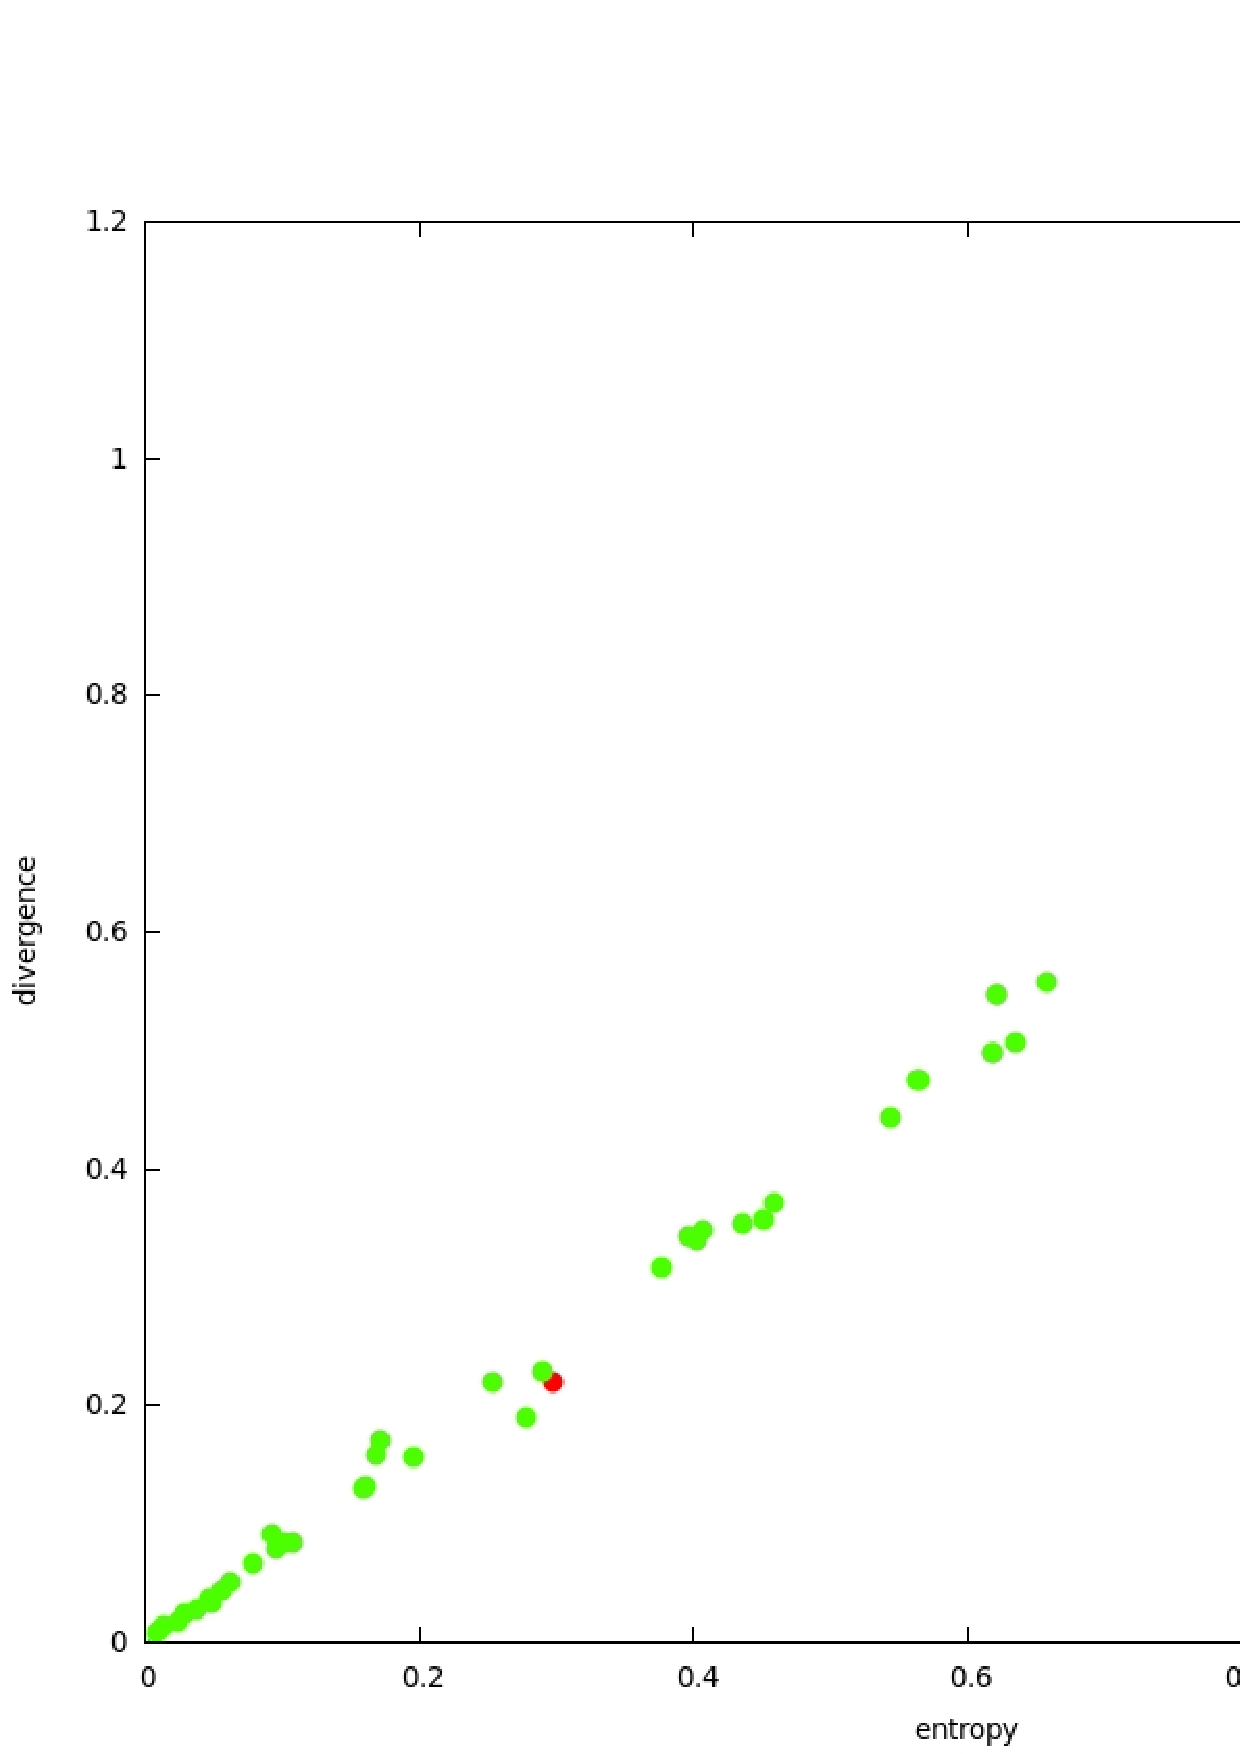
\includegraphics[width=12cm]{ATRIAL_FIBR/img/RRResults.jpg}
\end{figure}

